\documentclass[12pt,a4paper]{article}
\usepackage{fontspec}
\setmainfont{Noto Serif CJK SC}
\setsansfont{Noto Sans CJK SC}
\setmonofont{DejaVu Sans Mono}
\newfontfamily\heiti{Noto Sans CJK SC}
\XeTeXlinebreaklocale "zh"
\XeTeXlinebreakskip=0pt plus 1pt
\usepackage[left=3.17cm,right=3.17cm,top=2.54cm,bottom=2.54cm,footskip=1.25cm]{geometry}
\usepackage{amsmath,amssymb,graphicx,longtable,booktabs,array,calc}
\usepackage{titlesec,needspace,listings,xcolor}
\usepackage[hidelinks]{hyperref}
\setcounter{secnumdepth}{0}
\titleformat{\section}{\heiti\fontsize{14}{18}\selectfont\centering}{}{0pt}{}
\titleformat{\subsection}{\heiti\fontsize{12}{16}\selectfont}{}{0pt}{}
\titleformat{\subsubsection}{\heiti\fontsize{12}{16}\selectfont}{}{0pt}{}
\titlespacing*{\section}{0pt}{12pt}{6pt}
\titlespacing*{\subsection}{0pt}{9pt}{4pt}
\titlespacing*{\subsubsection}{0pt}{6pt}{3pt}
\setlength{\parindent}{2em}
\setlength{\parskip}{0pt}
\linespread{1}
\pagestyle{plain}
\pagenumbering{arabic}
\setlength{\emergencystretch}{4em}\sloppy
\setlength{\tabcolsep}{3pt}
\renewcommand{\arraystretch}{1.1}
\lstset{language=Python,basicstyle=\ttfamily\fontsize{9.5}{11}\selectfont,
numbers=left,numberstyle=\ttfamily\fontsize{7.5}{9}\selectfont,numbersep=5pt,
breaklines=true,breakatwhitespace=false,columns=fullflexible,keepspaces=true,
showstringspaces=false,tabsize=4,frame=lines,rulecolor=\color{black!30},
keywordstyle=\bfseries,commentstyle=\itshape\color{black!60},
aboveskip=6pt,belowskip=8pt,xleftmargin=12pt,
postbreak=\mbox{$\hookrightarrow$\space}}
\providecommand{\tightlist}{}
\errorcontextlines=100
\begin{document}
\begin{center}

\includegraphics[width=2.25cm]{assets/image1.png}\hspace{1.8cm}

\includegraphics[width=2.25cm]{assets/image2.jpg}\hspace{1.8cm}

\includegraphics[width=2.25cm]{assets/image3.jpg}

\vspace{12pt}
{\heiti\fontsize{18}{23}\selectfont 杭州电子科技大学}

\vspace{8pt}
{\heiti\fontsize{18}{23}\selectfont 2026 第八届新生数学建模竞赛}

\vspace{10pt}
{\heiti\fontsize{16}{20}\selectfont 题目　\underline{三维集成电路的多目标全局布线优化}}

\vspace{8pt}
{\heiti 摘　要}
\end{center}

芯片设计需要把分散的引脚接起来，但几条线如果选择同一条通道，就可能超过它能容纳的数量。本文把芯粒划成网格，用一棵树连接每组必须互通的引脚。在单层网格上同时控制线长和拥塞；在双层网格上，还需为每个跨层网络安排一个硅通孔（TSV），使它们的空间分布与给定热需求相匹配。

本文先给拥挤通道加价，用 A*
搜索逐个接入引脚，再撤下一部分既有线路重新寻找路径。双层问题先按槽位容量安排硅通孔，再比较换孔位置及其两侧线路的整体得分。

官方评分器的四个公开算例均通过合法性检查，平面总溢出均为零。二维两例线长为
1597 和 3787，得分 98.22 和 97.30。三维两例线长为 3218 和 6926，热匹配分
90.03 和 86.40，得分 83.97 和
82.82。全部四个隐藏算例合法，其中一个二维算例仍有 3
单位溢出。两问机器分分别为 87.46 和
76.33。对照实验显示，拥塞代价降低了溢出，过大的热权重则会因线长增加而降低综合分。

关键词　全局布线，斯坦纳树，拆线重布，硅通孔，热匹配

\clearpage\section{一、问题重述与分析}\label{ux4e00ux95eeux9898ux91cdux8ff0ux4e0eux5206ux6790}

把芯粒看成一张方格地图。每个网格单元（GCell）对应一个顶点，相邻单元之间的边对应一束可用通道。输入给出的每个网络是一组必须相互连通的引脚，同一个网络可以在中间顶点分叉，多条支路共用的那段边只计一次。当不同网络经过同一条边时，每个网络各占一份容量。因此，即使每个网络都找到了自己最短的路径，合在一起仍可能严重拥堵。

\subsection{1.1 二维问题}\label{ux4e8cux7ef4ux95eeux9898}

二维问题是在一张地图上为每个网络选出一棵树。容量为零的边相当于道路封闭。正容量边允许超额使用，但每超出一份都会影响得分。例如，两条网络经过容量为
1 的边，需求为 2，溢出为
1。分配好的网络越多，后续网络在短路径和空闲通道之间的取舍就越重要。

\subsection{1.2 双芯粒问题}\label{ux53ccux82afux7c92ux95eeux9898}

双芯粒可看作上下叠放的两张地图。同一平面坐标在两层上代表两个顶点，只有候选位置的硅通孔才能把它们连起来。每个跨层网络恰好使用一个
TSV。选定槽位后，可以在两层分别把引脚接到这个槽位，再用 TSV
把两棵树连起来。槽位太偏远会增加平面线长，槽位太集中又可能占满通道，还会改变热需求匹配。因此分配槽位时要先满足硬容量，再比较实际布线效果。

\section{二、模型假设与符号说明}\label{ux4e8cux6a21ux578bux5047ux8bbeux4e0eux7b26ux53f7ux8bf4ux660e}

布局、引脚和热需求均取自原始输入。每走一条平面边按 1 计长，每通过一个
TSV 按 6
计长，单位由赛题统一规定。多个引脚重合时，接到那个顶点即可。热图给定的是空间需求权重，评价时把同一热格内的
TSV 数与需求值逐格比较。计时从求解程序启动到退出。

\begin{center}\fontsize{12}{14.4}\selectfont 表1　集合、参数及变量\end{center}

\begingroup\fontsize{12}{14.4}\selectfont\begin{longtable}[]{@{}
  >{\raggedright\arraybackslash}p{(\columnwidth - 2\tabcolsep) * \real{0.5000}}
  >{\raggedright\arraybackslash}p{(\columnwidth - 2\tabcolsep) * \real{0.5000}}@{}}
\toprule\noalign{}
\begin{minipage}[b]{\linewidth}\raggedright
符号
\end{minipage} & \begin{minipage}[b]{\linewidth}\raggedright
定义
\end{minipage} \\
\midrule\noalign{}
\endhead
\bottomrule\noalign{}
\endlastfoot
\(N\)，\(P_n\) & 网络集，网络 \(n\) 的去重引脚集 \\
\(V\)，\(E_{\mathrm p}\)，\(E_{\mathrm t}\) & 节点集，输入平面边集，输入 TSV 边集 \\
\(c_e\)，\(\ell_e\) & 边容量，单位长度代价 \\
\(x_{ne}\)，\(y_{nv}\) & 是否使用边 \(e\)，是否包含节点 \(v\) \\
\(D_e\)，\(O_e\) & 边需求，平面边溢出 \\
\(h_b\)，\(t_b\) & 热格 \(b\) 的需求，分配的 TSV 数 \\
\(L_{\mathrm{ref}}\)，\(\tau\) & 输入参考线长，单算例时间上限 \\
\end{longtable}\endgroup

\section{三、数学模型}\label{ux4e09ux6570ux5b66ux6a21ux578b}

\subsection{3.1
从斯坦纳树到布线模型}\label{ux4eceux65afux5766ux7eb3ux6811ux5230ux5e03ux7ebfux6a21ux578b}

\subsubsection{3.1.1
为什么可以用树}\label{ux4e3aux4ec0ux4e48ux53efux4ee5ux7528ux6811}

普通最小生成树把给定顶点全部连起来。布线只要求引脚相通，因此允许选取额外网格点作分叉点，这对应图上的斯坦纳树。先固定其他网络和槽位，考虑某一网络的一组连通选边：若存在环，删去环上一边仍能保留引脚连通，而且会减少线长和边需求。跨层网络唯一的
TSV
必须连接两个芯粒，它不会落在这样的环上。因此用树描述布线与题设的合法性和优化方向一致。

每层正容量边构成一张有限图。若同层引脚都在同一连通分量，逐个沿路径接到已有连通子图就能把它们连齐，再删除环边可以得到一棵树。双层问题还需两层分量之间存在可用的
TSV
分配。这给出了建模可行性的图论解释，也说明为什么程序先筛选槽位再布线。

\subsubsection{3.1.2
连通性和树边数}\label{ux8fdeux901aux6027ux548cux6811ux8fb9ux6570}

记 $G=(V,E)$，$E=E_{\mathrm p}\cup E_{\mathrm t}$。取 $x_{ne},y_{nv}\in\{0,1\}$。对网络 $n$ 取一个引脚为根，令 \(x_{ne}\) 和 \(y_{nv}\)
分别表示是否选边和顶点。每个引脚顶点固定 \(y_{nv}=1\)。若边 \(e\) 的端点为
\(u\)、\(v\)，要求 \(x_{ne}\le y_{nu}\) 且 \(x_{ne}\le y_{nv}\)。对不含根的任意顶点集 \(U\) 和其中任一顶点
\(v\)，要求

\begin{equation}
\sum_{e\in\delta(U)}x_{ne}\ge y_{nv}
\label{eq:cut}
\end{equation}

\(\delta(U)\) 是一端在 \(U\) 内、另一端在 \(U\) 外的边集。若 \(U\)
中有选中顶点，至少有一条选中边向外。若一块选中顶点与根完全分离，取整块作
\(U\) 就会违反约束。

\begin{equation}
\sum_{e\in E}x_{ne}=\sum_{v\in V}y_{nv}-1
\label{eq:tree}
\end{equation}

连通已由割约束保证，再将选边数固定为选点数减一即可排除环。所有引脚重合时，单顶点和零条边也满足该等式。零容量边固定为不选，边集只含输入列出的边。

\subsection{3.2
共享容量与跨层约束}\label{ux5171ux4eabux5bb9ux91cfux4e0eux8de8ux5c42ux7ea6ux675f}

\subsubsection{3.2.1
平面边的需求和溢出}\label{ux5e73ux9762ux8fb9ux7684ux9700ux6c42ux548cux6ea2ux51fa}

\begin{equation}
D_e=\sum_{n\in N}x_{ne}
\label{eq:demand}
\end{equation}

每个使用边 \(e\) 的网络为需求贡献
1。同网内部共用的一段路径已经由一个二元变量表示，无需重复计算。

\begin{equation}
O_e=\max\{0,D_e-c_e\}
\label{eq:overflow}
\end{equation}

该式用于正容量平面边。需求大于容量时，差值进入评分。容量为零的边禁止使用，因此也不参加归一化。

\subsubsection{3.2.2
硅通孔的数量与硬容量}\label{ux7845ux901aux5b54ux7684ux6570ux91cfux4e0eux786cux5bb9ux91cf}

\begin{equation}
\sum_{e\in E_{\mathrm t}}x_{ne}=k_n-1
\label{eq:tsv-count}
\end{equation}

\(k_n\)
是网络引脚所占的芯粒层数，$k_n\in\{1,2\}$。单层网络的右端为零，且另一层顶点固定不选。跨层网络的右端为一，两侧平面树通过唯一的
TSV 相连。

\begin{equation}
D_e\le c_e,\qquad e\in E_{\mathrm t}
\label{eq:tsv-cap}
\end{equation}

每个已选 TSV 槽位都必须遵守容量上限。题设规定有引脚的 GCell
不设候选槽位，程序直接读取输入中的槽位。

\subsection{3.3
评分指标及其含义}\label{ux8bc4ux5206ux6307ux6807ux53caux5176ux542bux4e49}

\subsubsection{3.3.1 线长与拥塞}\label{ux7ebfux957fux4e0eux62e5ux585e}

\begin{equation}
L=\sum_{n\in N}\sum_{e\in E}\ell_e x_{ne}
\label{eq:length}
\end{equation}

\(L\) 汇总所有网络的选边长度。每条平面边计 1，每个 TSV 计 6。

\begin{equation}
W=100\exp\left[-4\max\left\{0,\frac{L}{L_{\mathrm{ref}}}-1\right\}\right]
\label{eq:wire}
\end{equation}

参考线长由题方提供，忽略容量、障碍与槽位竞争，端点超过 12
个时可能用近似值。超过参考值越多，线长分越低。题面未定义零参考值时的公式，本地按参考值趋近零的右极限处理。

\begin{equation}
C=\frac{100}{\sqrt{1+10\displaystyle\sum_{\substack{e\in E_{\mathrm p}\\c_e>0}}\left(\frac{O_e}{c_e}\right)^2}}
\label{eq:congestion}
\end{equation}

无溢出时 \(C\) 为 100。若只有一条容量为 1 的边溢出 1 单位，\(C\) 约为
30.15。若同样的溢出出现在容量为 2 的边，\(C\) 约为
53.45。这个例子解释了程序为何优先消除小容量边上的拥塞。

\subsubsection{3.3.2
热格归类与相关性}\label{ux70edux683cux5f52ux7c7bux4e0eux76f8ux5173ux6027}

\begin{equation}
b=\left\lfloor\frac{B_y y}{n_y}\right\rfloor B_x+\left\lfloor\frac{B_x x}{n_x}\right\rfloor
\label{eq:bin}
\end{equation}

\(B_x\) 和 \(B_y\) 分别是热图两个方向的分格数，\(n_x\) 和 \(n_y\)
是布线网格尺寸。先求行列号，再把行列号合成连续的热格编号 \(b\)。

\begin{equation}
t_b=\sum_{\substack{e\in E_{\mathrm t}\\\operatorname{bin}(e)=b}}D_e
\label{eq:counts}
\end{equation}

把落入同一热格的槽位使用次数相加得到
\(t_b\)。这一步可以直接从路线和槽位坐标重算。

\begin{equation}
\rho=\frac{\sum_b(h_b-\bar h)(t_b-\bar t)}{\sqrt{\sum_b(h_b-\bar h)^2\sum_b(t_b-\bar t)^2}}
\label{eq:pearson}
\end{equation}

\(h_b\) 是该热格的需求。减去均值后，若高需求位置通常同时有较多
TSV，分子倾向于为正。分母把结果归一化到 \(-1\) 与 1
之间。任一向量在各格都相同时按赛题取 \(\rho=0\)。

\begin{equation}
H=50(1+\rho)
\label{eq:heat}
\end{equation}

该式把相关性映射为百分制。\(H=50\) 对应零相关，\(H\) 越高表示空间匹配越强。

\subsubsection{3.3.3
运行时间与综合分}\label{ux8fd0ux884cux65f6ux95f4ux4e0eux7efcux5408ux5206}

\begin{equation}
T=\min\left\{100,\max\left\{0,\frac{100\log_{10}(\tau/t)}{\log_{10}(\tau/10)}\right\}\right\}
\label{eq:time}
\end{equation}

\(\tau\) 是该例时限，\(t\) 是实际耗时。10 秒内 \(T\) 取 100，到达时限时 \(T\) 为 0。

\begin{equation}
S^{(1)}=0.55W+0.35C+0.10T
\label{eq:score1}
\end{equation}

二维评分只用线长、拥塞和时间。

\begin{equation}
S^{(2)}=0.45W+0.25C+0.20H+0.10T
\label{eq:score2}
\end{equation}

三维把热匹配纳入评分。两问都先检查合法性和资源限制，违规时单例计零分。每问的机器分由公开均分和隐藏均分分别按
0.4 与 0.6 加权。

\section{四、算法设计与独立验证}\label{ux56dbux7b97ux6cd5ux8bbeux8ba1ux4e0eux72ecux7acbux9a8cux8bc1}

\subsection{4.1
加权最短路与多端点树}\label{ux52a0ux6743ux6700ux77edux8defux4e0eux591aux7aefux70b9ux6811}

\subsubsection{4.1.1
给共享通道设定代价}\label{ux7ed9ux5171ux4eabux901aux9053ux8bbeux5b9aux4ee3ux4ef7}

令 \(u_e\) 为已占用通道数，\(r_e=\frac{u_e}{c_e}\)。在方案 B 至 E 中，将边权设为下式。\(\gamma\) 默认
18。\(h_e\) 初始为零，每轮在溢出边上加
\(0.4\gamma\)。即将达到容量时，使用下一条网络的代价增大；历史项让反复拥堵的边更难入选。方案
A 的边权恒为 1。

\begin{equation}
w_e=1+0.4r_e^2+\gamma\max\left\{0,r_e-\frac{c_e-1}{c_e}\right\}+h_e
\label{eq:weight}
\end{equation}

基础代价 1
对应平面边长。第二项随利用率上升，第三项在通道满载后提高再占用的代价，最后一项记录以往出现的溢出。

式\eqref{eq:weight}的实现与默认参数见附录5.4。

\subsubsection{4.1.2 用 A*
接入新的引脚}\label{ux7528-a-ux63a5ux5165ux65b0ux7684ux5f15ux811a}

程序先取一个引脚作起点，从离当前树最近的未接引脚出发寻找接入路径。这里的距离为横向坐标差与纵向坐标差绝对值之和，即曼哈顿距离。A*
按已走代价与剩余代价下界之和选择下一步。剩余下界取到包住当前树的最小矩形的距离：接到树必先到达该矩形，而每步的代价至少为
1。相邻顶点到矩形的距离最多相差 1，因此启发式一致{[}1{]}。

\begin{equation}
\eta(x,y)=\max\{x_0-x,0,x-x_1\}+\max\{y_0-y,0,y-y_1\}.
\label{eq:astar}
\end{equation}
式\eqref{eq:astar}中，$[x_0,x_1]\times[y_0,y_1]$ 为当前树的包围盒。搜索优先级为 $g+\eta$，其中 $g$ 为已走边权之和。A* 搜索、路径回溯和多端点接入共用附录5.2的完整函数。

找到新路径与树的第一个接触点时停止搜索。新路径只在这个点接入，因此不会形成环。举例说，三个引脚位于
\((0,0)\)、\((2,0)\)、\((1,1)\)，在无障碍等权网格上，选择坐标中位点 \((1,0)\)
作分叉点，三段共 3
条边。程序在处理三个端点时也试算这个中位点，并用实际边权比较。更多端点时，精确求解斯坦纳树的复杂度随端点数迅速增加{[}2{]}，逐次接入便于把时间控制在评分要求内。

\subsection{4.2
容量匹配和热匹配}\label{ux5bb9ux91cfux5339ux914dux548cux70edux5339ux914d}

\subsubsection{4.2.1
初始槽位的可行性}\label{ux521dux59cbux69fdux4f4dux7684ux53efux884cux6027}

初始分配先排除无法接通的槽位。每层仅使用正容量边，把任意两点之间可以互达的区域称为连通分量。槽位的两端必须分别落在两层引脚所在的分量中。通过这项筛选后，用槽位到两层引脚包围盒的距离和排序，再用到两层最近引脚的距离打破并列。

如果最合适的槽位已满，直接跳过可能让后面的网络无处可选。设网络甲只能用槽位一，网络乙已占槽位一但也能用槽位二，且槽位二有空位。把乙迁到槽位二便能为甲腾出空间。程序通过增广路径在多个网络和槽位之间寻找这样的迁移链。

\subsubsection{4.2.2
换槽后的整体比较}\label{ux6362ux69fdux540eux7684ux6574ux4f53ux6bd4ux8f83}

重布跨层网时，候选包括原槽位、几何排序最靠前的至多三个有余量槽位，以及启用热项时按几何与热收益混合排序的至多三个槽位。混合排序用包围盒距离加
0.05 倍最近引脚距离，再减去
\(\frac{2.5\lambda\max(L_{\mathrm{ref}},1)H}{200}\)。这个估计只用于缩小搜索范围。为每个候选算出两侧平面树后，用实际全局质量
\(0.45W+0.25C+0.20\lambda H\) 作选择。\(\lambda=0\)
时只看线长和拥塞，报告实验结果仍使用官方权重。

\begin{equation}
R(s)=d(s)+0.05p(s)-\frac{2.5\lambda\max(L_{\mathrm{ref}},1)}{200}H(s).
\label{eq:rank}
\end{equation}
式\eqref{eq:rank}用于候选截取。$d(s)$ 为两层包围盒距离之和，$p(s)$ 为到两层最近引脚的距离之和，$H(s)$ 为撤去当前网络后再加入槽位 $s$ 得到的热分。初始候选按 $(d,p,s)$ 排序，容量匹配见附录5.3。
\begin{equation}
Q_{\lambda}=0.45W+0.25C+0.20\lambda H.
\label{eq:quality}
\end{equation}
式\eqref{eq:quality}在默认 $\lambda=1$ 时对应三维质量项，求解器用它比较换槽后的完整路径。附录5.4中的 \texttt{quality} 和 \texttt{score\_for} 分别实现质量比较与热格缓存。二维候选使用 $0.55W+0.35C$。时间分由运行后单独计量。
\subsection{4.3
拆线重布及校验}\label{ux62c6ux7ebfux91cdux5e03ux53caux6821ux9a8c}

较长的网络通常需要跨过更多区域，故方案 C、D、E
先按各层引脚包围盒跨度之和排序，以引脚数打破并列，均从大到小。基线 A
和只加拥塞权重的 B 沿用输入顺序。D 至多重布三轮，E
默认至多七轮，并在重布时优先处理沿途溢出量较大的网络。

每次先撤掉一个网络的旧路径，把它占用的容量归还，再在其他网络仍在原位的条件下试算新路径。拥塞较重时，允许个别轮次暂时绕开满载边以腾出通道。每轮结束保留目前质量最高的完整解，达到轮数、停止条件或用时保护线后输出。反复拥塞的边在后续轮次中获得历史加价，这一思路与协商式布线有关{[}3{]}。

拆线重布及完整解保留见附录5.4，独立验证见附录5.5。式\eqref{eq:pearson}、\allowbreak\eqref{eq:score1}和\allowbreak\eqref{eq:score2}对应附录5.5中的热分与评分函数。验证程序与求解器分别工作。它从 JSON
重新读入每个网络的边，先检查未知边、重复边和禁行边，再从一个引脚沿这些边逐层访问顶点。访问结果必须覆盖所有引脚和所选边的端点，且满足树边数条件。最后重新统计两层通道和
TSV 槽位占用，依照题目公式算分。公开结果还与原版评分器的输出相互核对。


\begin{center}
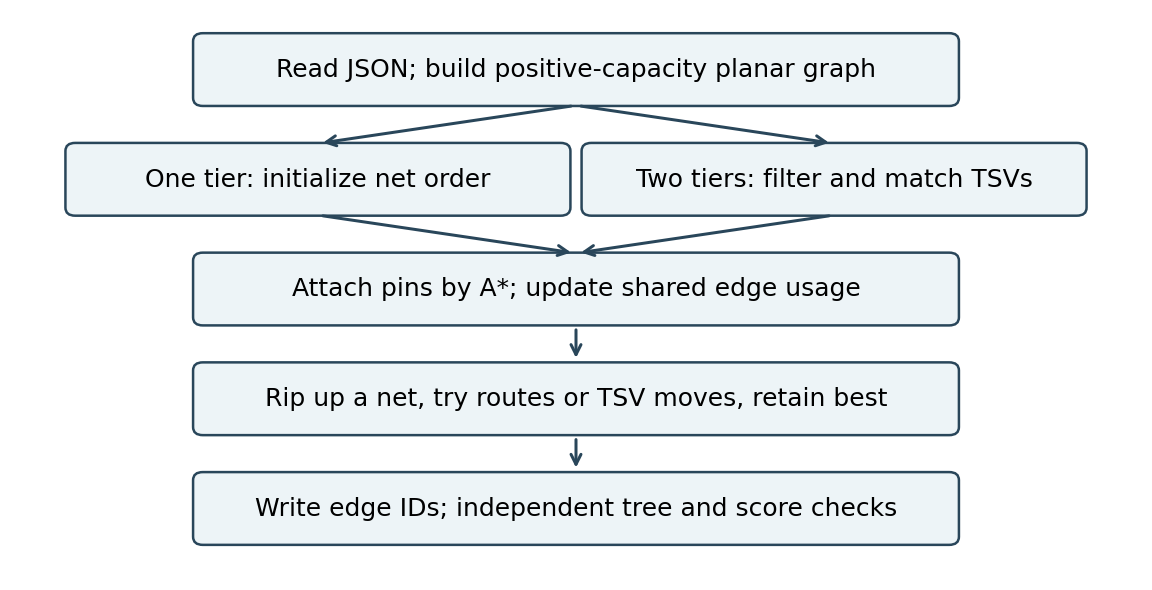
\includegraphics[width=5.11811in,height=2.62125in]{assets/image4.png}

{\fontsize{12}{14.4}\selectfont 图1　容量匹配、成树、重布与验证流程}
\end{center}


\section{五、实验设计与结果}\label{ux4e94ux5b9eux9a8cux8bbeux8ba1ux4e0eux7ed3ux679c}

\subsection{5.1
数据及计量环境}\label{ux6570ux636eux53caux8ba1ux91cfux73afux5883}

实验从简单方案逐项加入改动。A 用等权路径，B 补上拥塞权重，\(C\)
再调整处理顺序，D 加入重布，E
同时使用交替起点、三端点中位候选和双层换槽。双层另设不使用热项的 cold
组，以观察相同任务加入热目标后的变化。二维公开算例有 230 和 520
个网络，双层有 300 和 600 个网络。评分器 2.0.0 在 Linux 的 Wine 10.0
兼容层中调用 Windows Python
3.12.10。表2的时间与内存来自原版评分器，其他实验的内存是本地每 5
毫秒采样所得的进程常驻内存峰值。

\subsection{5.2
官方成绩及误差来源}\label{ux5b98ux65b9ux6210ux7ee9ux53caux8befux5deeux6765ux6e90}

\begin{center}\fontsize{12}{14.4}\selectfont 表2　官方评分器运行结果\end{center}

\begingroup\fontsize{12}{14.4}\selectfont\begin{longtable}[]{@{}
  >{\raggedright\arraybackslash}p{(\columnwidth - 12\tabcolsep) * \real{0.1429}}
  >{\raggedright\arraybackslash}p{(\columnwidth - 12\tabcolsep) * \real{0.1429}}
  >{\raggedright\arraybackslash}p{(\columnwidth - 12\tabcolsep) * \real{0.1429}}
  >{\raggedright\arraybackslash}p{(\columnwidth - 12\tabcolsep) * \real{0.1429}}
  >{\raggedright\arraybackslash}p{(\columnwidth - 12\tabcolsep) * \real{0.1429}}
  >{\raggedright\arraybackslash}p{(\columnwidth - 12\tabcolsep) * \real{0.1429}}
  >{\raggedright\arraybackslash}p{(\columnwidth - 12\tabcolsep) * \real{0.1429}}@{}}
\toprule\noalign{}
\begin{minipage}[b]{\linewidth}\raggedright
算例
\end{minipage} & \begin{minipage}[b]{\linewidth}\raggedright
\(L\)
\end{minipage} & \begin{minipage}[b]{\linewidth}\raggedright
总/最大溢出
\end{minipage} & \begin{minipage}[b]{\linewidth}\raggedright
\(H\)
\end{minipage} & \begin{minipage}[b]{\linewidth}\raggedright
秒
\end{minipage} & \begin{minipage}[b]{\linewidth}\raggedright
MB
\end{minipage} & \begin{minipage}[b]{\linewidth}\raggedright
得分
\end{minipage} \\
\midrule\noalign{}
\endhead
\bottomrule\noalign{}
\endlastfoot
Q1\_P1 & 1597 & 0/0 & --- & 0.65 & 15.3 & 98.22 \\
Q1\_P2 & 3787 & 0/0 & --- & 0.95 & 18.1 & 97.30 \\
Q1\_H1 & 7936 & 0/0 & --- & 1.87 & 19.7 & 90.50 \\
Q1\_H2 & 4037 & 3/1 & --- & 1.17 & 17.8 & 70.68 \\
Q2\_P1 & 3218 & 0/0 & 90.03 & 1.73 & 22.0 & 83.97 \\
Q2\_P2 & 6926 & 0/0 & 86.40 & 5.13 & 45.3 & 82.82 \\
Q2\_H1 & 9704 & 0/0 & 54.66 & 6.16 & 31.5 & 64.27 \\
Q2\_H2 & 9552 & 0/0 & 97.79 & 10.70 & 50.5 & 78.97 \\
\end{longtable}\endgroup

\begin{center}\fontsize{12}{14.4}\selectfont 表2及摘要保留原始官评轮次的成绩。专项核验再次执行原版评分器，记录单独保存，耗时变化会影响时间分。表2中，两个二维公开例分别比参考线长多 0.82\% 和 1.26\%，双层公开例分别多\end{center}
9.34\% 和 9.69\%。四个公开例均无溢出，两个双层例分别布置了 130 和 295 个
TSV。二维隐藏例 Q1\_H2 的三条边各溢出 1
单位，其余七例均无溢出。八例都通过合法性检查和资源限制。Q2\_H1
虽无溢出，线长分只有 40.74，热匹配分为
54.66。这说明消除拥塞之后，槽位与路径的选择仍可能明显影响得分。

\subsection{5.3
算法对照与路线图}\label{ux7b97ux6cd5ux5bf9ux7167ux4e0eux8defux7ebfux56fe}

\begin{center}\fontsize{12}{14.4}\selectfont 表3　各算法公开算例本地综合分\end{center}

\begingroup\fontsize{12}{14.4}\selectfont\begin{longtable}[]{@{}
  >{\raggedright\arraybackslash}p{(\columnwidth - 8\tabcolsep) * \real{0.2000}}
  >{\raggedright\arraybackslash}p{(\columnwidth - 8\tabcolsep) * \real{0.2000}}
  >{\raggedright\arraybackslash}p{(\columnwidth - 8\tabcolsep) * \real{0.2000}}
  >{\raggedright\arraybackslash}p{(\columnwidth - 8\tabcolsep) * \real{0.2000}}
  >{\raggedright\arraybackslash}p{(\columnwidth - 8\tabcolsep) * \real{0.2000}}@{}}
\toprule\noalign{}
\begin{minipage}[b]{\linewidth}\raggedright
方案
\end{minipage} & \begin{minipage}[b]{\linewidth}\raggedright
Q1\_P1
\end{minipage} & \begin{minipage}[b]{\linewidth}\raggedright
Q1\_P2
\end{minipage} & \begin{minipage}[b]{\linewidth}\raggedright
Q2\_P1
\end{minipage} & \begin{minipage}[b]{\linewidth}\raggedright
Q2\_P2
\end{minipage} \\
\midrule\noalign{}
\endhead
\bottomrule\noalign{}
\endlastfoot
A & 59.51 & 58.64 & 57.38 & 55.75 \\
B & 92.15 & 84.50 & 79.39 & 67.22 \\
\(C\) & 80.18 & 91.95 & 80.12 & 77.64 \\
D & 92.39 & 94.32 & 80.72 & 78.42 \\
E & 98.22 & 97.30 & 83.97 & 82.82 \\
cold & --- & --- & 82.98 & 81.38 \\
\end{longtable}\endgroup

B 把四例总溢出由 63、120、45、108 降为
0、1、0、1。排序单独加入后，Q1\_P1 的溢出由 0 变为 1，得分从 92.15 降到
80.18；Q1\_P2 则由 84.50 升为
91.95。按跨度优先让较长网络先选择通道，但顺序仍会改变后续网络可用的通道。E
在四例的分数均高于 D，输出的公开路线与官方评分器产生的文件逐字节一致。


\begin{center}
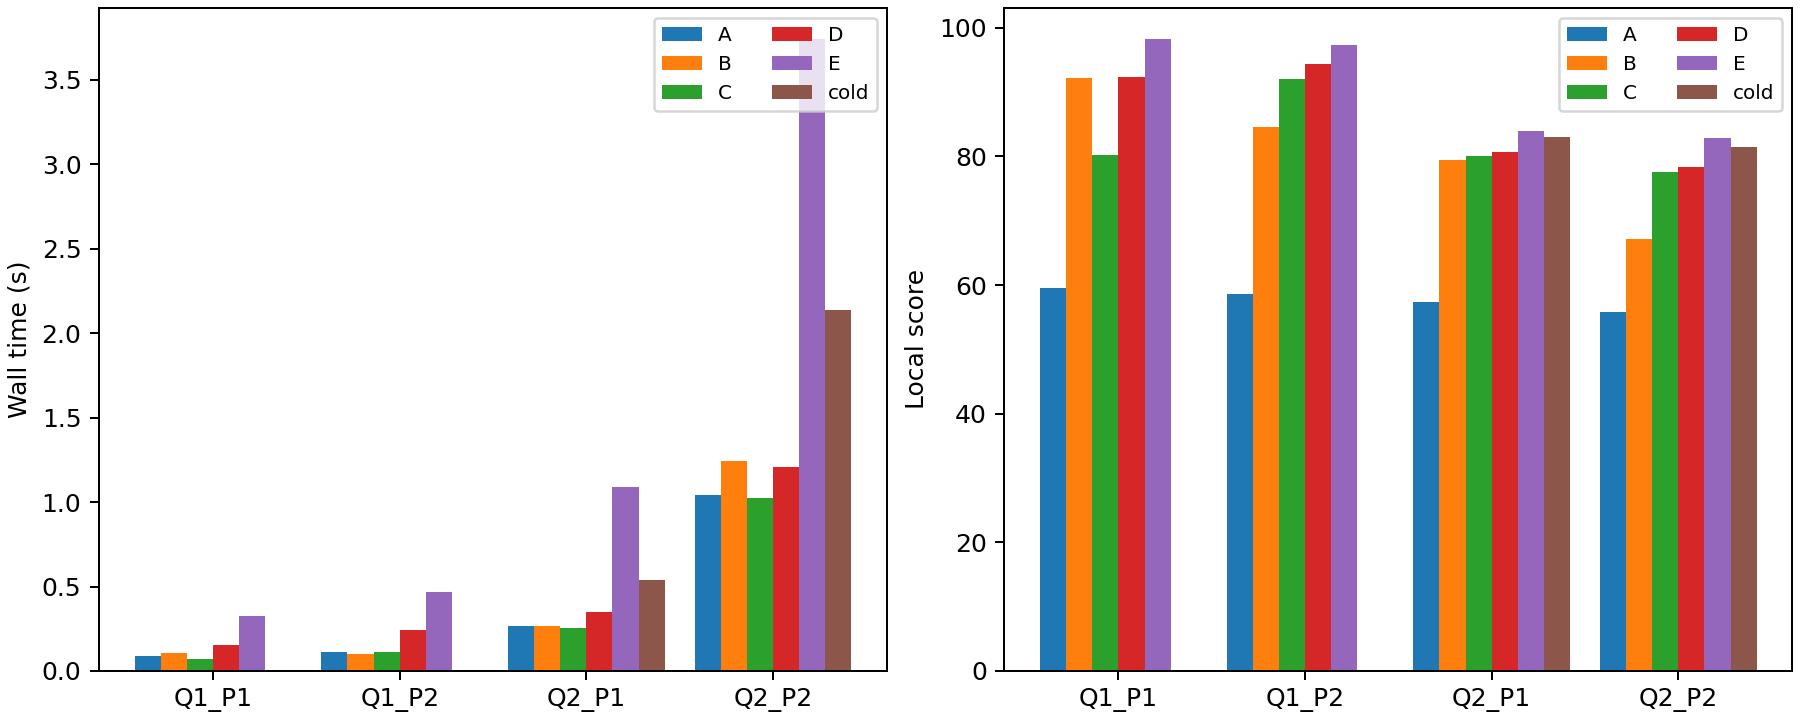
\includegraphics[width=5.51181in,height=2.20472in]{assets/image5.png}

{\fontsize{12}{14.4}\selectfont 图2　公开算例本地运行时间与算法得分}
\end{center}



\begin{center}
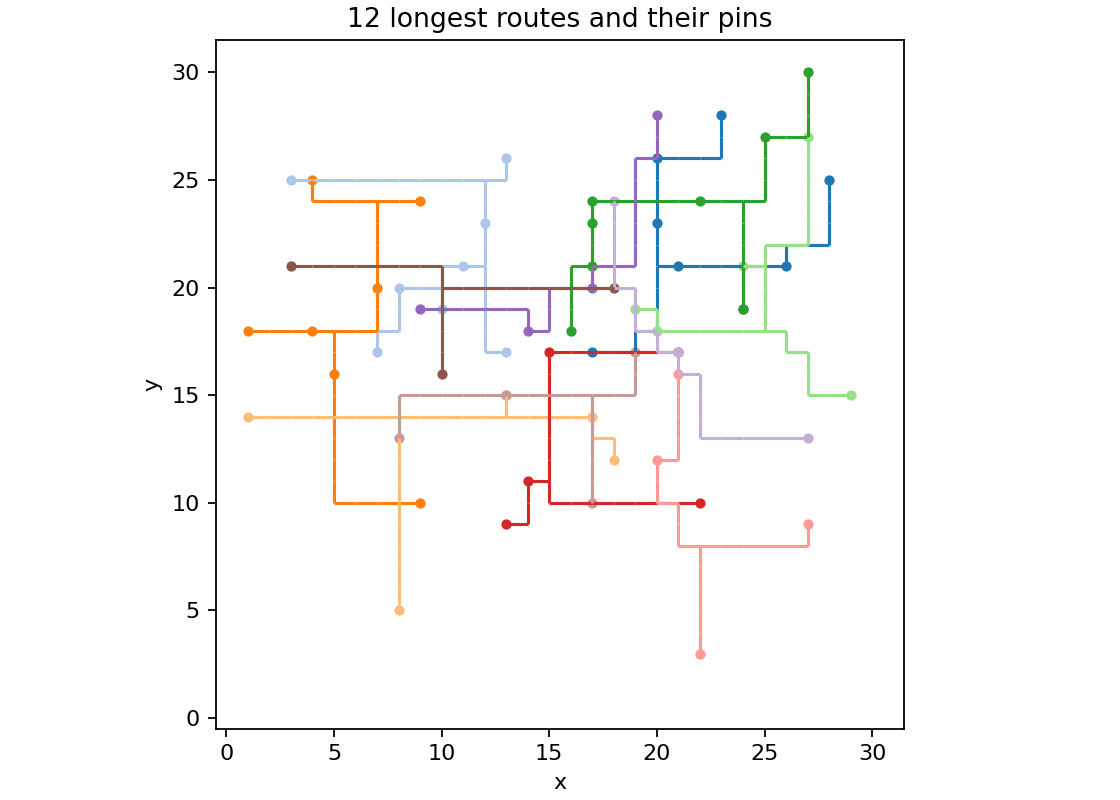
\includegraphics[width=4.33071in,height=3.09336in]{assets/image6.png}

{\fontsize{12}{14.4}\selectfont 图3　Q1\_P1 线长前十二个网络的路径与引脚}
\end{center}



\begin{center}
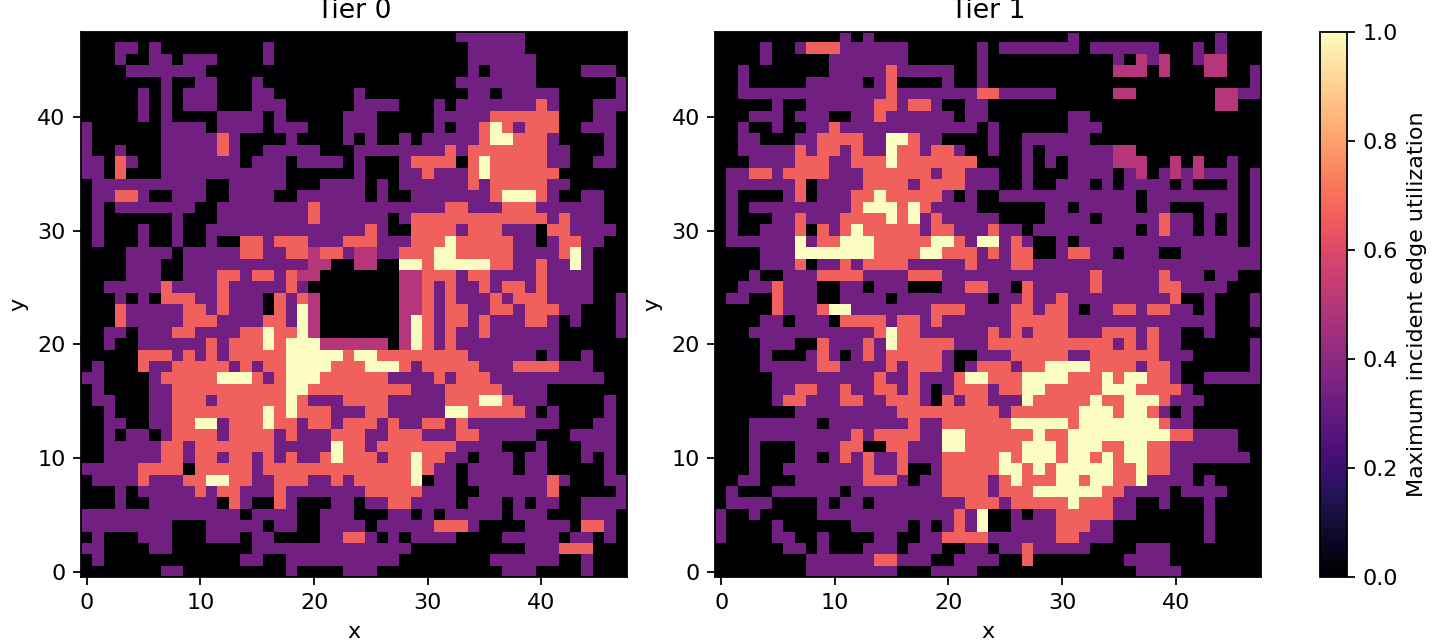
\includegraphics[width=5.51181in,height=2.44969in]{assets/image7.png}

{\fontsize{12}{14.4}\selectfont 图4　Q2\_P2 两芯粒的 GCell 容量利用率}
\end{center}


图3和图5用不同颜色区分网络，圆点表示引脚。图5的竖向线段表示连接两层的
TSV。图4显示每个网格单元相邻平面边中最大的需求容量比，接近 1
的位置意味着至少一条相邻边已接近满载。


\begin{center}
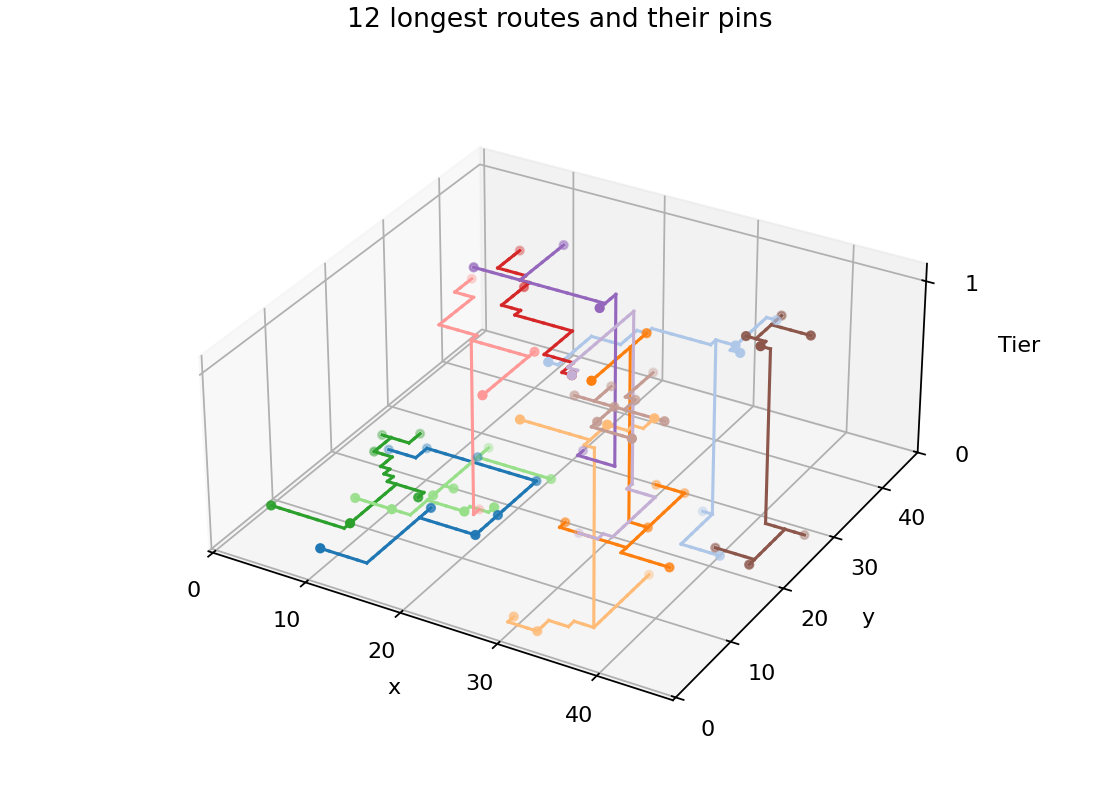
\includegraphics[width=4.33071in,height=3.09336in]{assets/image8.png}

{\fontsize{12}{14.4}\selectfont 图5　Q2\_P2 的十二条较长网络与跨层连接}
\end{center}


\section{六、敏感性分析}\label{ux516dux654fux611fux6027ux5206ux6790}

\subsection{6.1
平面拥塞权重与迭代次数}\label{ux5e73ux9762ux62e5ux585eux6743ux91cdux4e0eux8fedux4ee3ux6b21ux6570}

固定原始输入与官方计分公式，仅改变求解参数。二维的 \(\gamma\) 使用 4、10、18 和
32，两个算例在七轮下均为零溢出，Q1\_P1 分数范围为 98.09--98.22，Q1\_P2
为 97.30--97.47。固定 \(\gamma=18\)，将迭代次数从 0、1、3 增至
7，两例均有持续改善。进一步迭代会增加耗时，接近 10
秒后需要把增益与时间扣分一并衡量。

\subsection{6.2
线长与热匹配的取舍}\label{ux7ebfux957fux4e0eux70edux5339ux914dux7684ux53d6ux820d}

开启热项使 Q2\_P1 的 \(H\) 从 81.87 升至 90.03，线长增加 15；Q2\_P2 的 \(H\) 从
74.51 升至 86.40，线长增加 48。二者综合分分别提高约 0.99 和 1.44。令 \(\lambda=4\)
时 \(H\) 上升至 97.47 和 94.98，但线长升至 3332 和 7154，最终分下降。\(\lambda=0.5\)
在 Q2\_P2 得 82.99，高于默认值的 82.82；\(\lambda=1\) 在 Q2\_P1
的表现更好。正式求解保持同一 \(\lambda=1\)。


\begin{center}
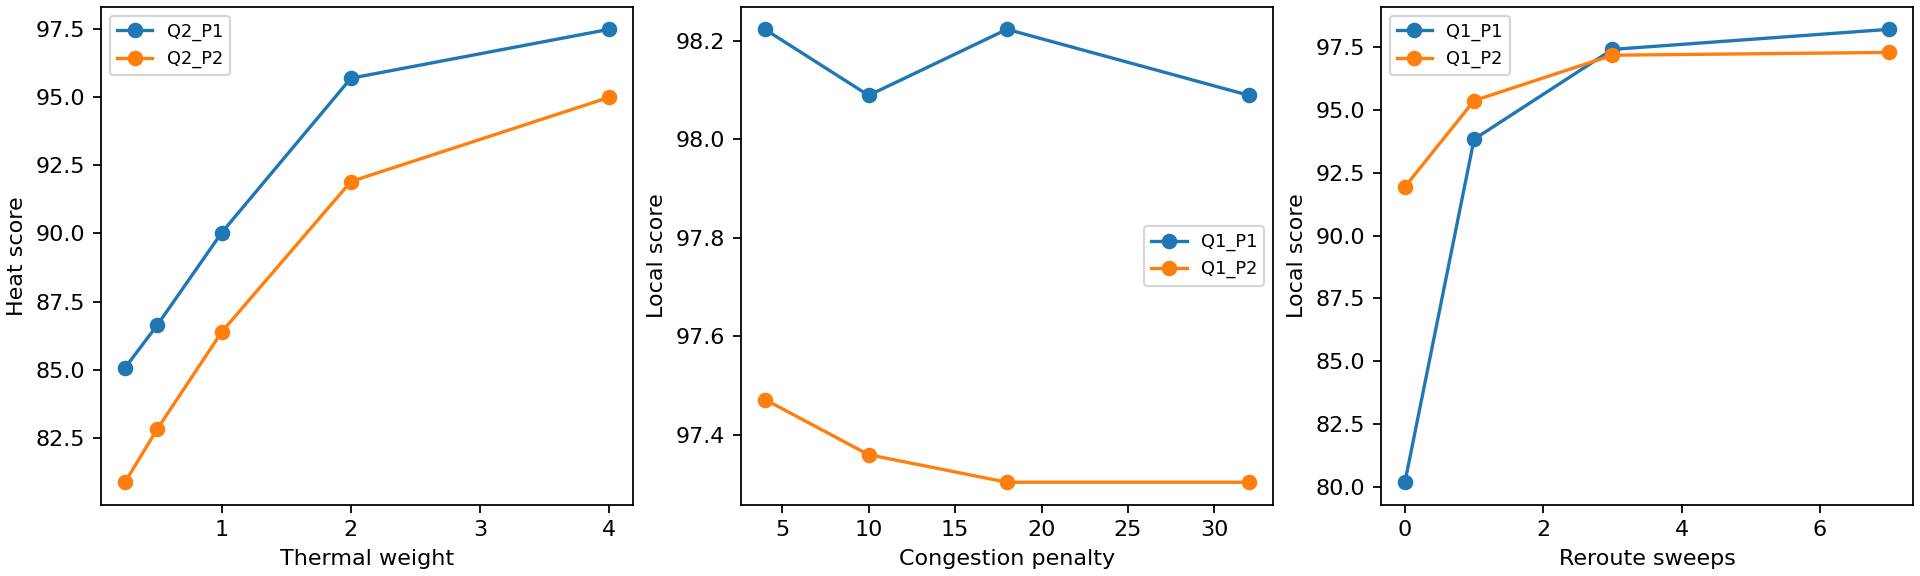
\includegraphics[width=5.51181in,height=1.65354in]{assets/image9.png}

{\fontsize{12}{14.4}\selectfont 图6　热权重、拥塞惩罚和重布轮次的独立敏感性实验}
\end{center}


\section{七、模型评价与局限}\label{ux4e03ux6a21ux578bux8bc4ux4ef7ux4e0eux5c40ux9650}

自建 \(80\times73\times2\) 的 800 网络算例，含单引脚和 13 引脚网络、容量为 2 的
TSV、\(7\times5\) 热图及禁边。固定随机种子 202611，算法在 5.55
秒通过独立校验，线长 8863、总溢出
0。自建算例的参考值仅用于运行测试，其综合分不纳入正式比较。

单次 A*
最坏会访问一个芯粒内全部可达的顶点，跨层网络与槽位的数目同时增大时，候选表空间也会随两者乘积增长。本例用稀疏邻接表保存实际可走的边，并把重布限制在少量候选上。求解器只根据输入给出的大小、引脚、边和容量运行，因此矩形网格、不同热图和多容量槽位共用同一个流程。

网络顺序会影响早期留下的可用通道，逐网调整也可能停在局部最优。例如，两条网络若分别换槽都变差，同时交换槽位却有机会缩短总线。这类组合不在目前的搜索范围。包围盒距离只提供几何估计，存在障碍时可能漏掉实际代价较低的槽位。后续可对拥堵边周围的网络做成组重布，并在少引脚小区域内比较精确子树。热分衡量的是空间相关性，若要估计实际温升，还需材料、功率和边界条件。

\section{八、结果诊断与有效性检查}\label{ux516bux7ed3ux679cux8bcaux65adux4e0eux6709ux6548ux6027ux68c0ux67e5}

\subsection{8.1
二维通道的使用情况}\label{ux4e8cux7ef4ux901aux9053ux7684ux4f7fux7528ux60c5ux51b5}

\subsubsection{8.1.1
从路线重算边使用次数}\label{ux4eceux8defux7ebfux91cdux7b97ux8fb9ux4f7fux7528ux6b21ux6570}

总溢出为零只能说明容量没有被突破。若很多边恰好满载，新增一条网络仍可能让局部拥塞。为同时观察这两点，表4读取四份公开输入和对应算法输出，对正容量平面边区分已用、满载和超载。满载指需求等于容量，超载指需求大于容量，两列互斥。

\begin{center}\fontsize{12}{14.4}\selectfont 表4　初始等权算法和综合算法的平面通道占用\end{center}

\begingroup\fontsize{12}{14.4}\selectfont\begin{longtable}[]{@{}
  >{\raggedright\arraybackslash}p{(\columnwidth - 10\tabcolsep) * \real{0.1667}}
  >{\raggedright\arraybackslash}p{(\columnwidth - 10\tabcolsep) * \real{0.1667}}
  >{\raggedright\arraybackslash}p{(\columnwidth - 10\tabcolsep) * \real{0.1667}}
  >{\raggedright\arraybackslash}p{(\columnwidth - 10\tabcolsep) * \real{0.1667}}
  >{\raggedright\arraybackslash}p{(\columnwidth - 10\tabcolsep) * \real{0.1667}}
  >{\raggedright\arraybackslash}p{(\columnwidth - 10\tabcolsep) * \real{0.1667}}@{}}
\toprule\noalign{}
\begin{minipage}[b]{\linewidth}\raggedright
算例
\end{minipage} & \begin{minipage}[b]{\linewidth}\raggedright
方案
\end{minipage} & \begin{minipage}[b]{\linewidth}\raggedright
正容量边
\end{minipage} & \begin{minipage}[b]{\linewidth}\raggedright
已用边
\end{minipage} & \begin{minipage}[b]{\linewidth}\raggedright
满载边
\end{minipage} & \begin{minipage}[b]{\linewidth}\raggedright
超载边
\end{minipage} \\
\midrule\noalign{}
\endhead
\bottomrule\noalign{}
\endlastfoot
Q1\_P1 & A & 1913 & 1004 & 108 & 47 \\
Q1\_P1 & E & 1913 & 1125 & 52 & 0 \\
Q1\_P2 & A & 4240 & 2203 & 120 & 82 \\
Q1\_P2 & E & 4240 & 2493 & 47 & 0 \\
Q2\_P1 & A & 3884 & 1720 & 132 & 33 \\
Q2\_P1 & E & 3884 & 1925 & 57 & 0 \\
Q2\_P2 & A & 8753 & 3564 & 264 & 86 \\
Q2\_P2 & E & 8753 & 4018 & 130 & 0 \\
\end{longtable}\endgroup

\subsubsection{8.1.2
为什么先处理溢出}\label{ux4e3aux4ec0ux4e48ux5148ux5904ux7406ux6ea2ux51fa}

对所有正容量平面边，将归一化溢出的平方求和记为 \(q\)，则拥塞分随 \(q\)
单调降低。把某条边的溢出从 \(o\) 减到 \(o-1\) 时，\(q\) 的下降量为

\begin{equation}
\Delta q=\frac{o^2-(o-1)^2}{c_e^2}=\frac{2o-1}{c_e^2}
\label{eq:delta}
\end{equation}

这个下降量随原溢出 \(o\) 增大，也随容量 \(c_e\)
减小而增大。重布中优先访问溢出大的网络，可尽快试探能否解除这些冲突。若一条新路径减少本边拥塞，却在另一条容量更小的边上增加溢出，最终仍以全局的拥塞分和线长分判断。

\begin{center}\fontsize{12}{14.4}\selectfont 表4的综合算法在四例中均已消除超载。满载边依然存在，这与图4中的高利用率位置相符。若实际设计要求预留备用容量，应另设通道余量目标，并用新的目标重新验证。\end{center}

\subsection{8.2
双层热格的布置差异}\label{ux53ccux5c42ux70edux683cux7684ux5e03ux7f6eux5deeux5f02}

\subsubsection{8.2.1 从 TSV
边恢复热格计数}\label{ux4ece-tsv-ux8fb9ux6062ux590dux70edux683cux8ba1ux6570}

热图匹配的改变可以从路线结果直接追溯。表5选取
Q2\_P2，把冷方案与综合方案的 TSV
边端点按公式投影到热格，再统计每格的槽位使用次数。格坐标从零开始。差值表示综合方案相对于冷方案的使用次数变化。

\begin{center}\fontsize{12}{14.4}\selectfont 表5　Q2\_P2 各热格需求与 TSV 计数\end{center}

\begingroup\fontsize{12}{14.4}\selectfont\begin{longtable}[]{@{}
  >{\raggedright\arraybackslash}p{(\columnwidth - 8\tabcolsep) * \real{0.2000}}
  >{\raggedright\arraybackslash}p{(\columnwidth - 8\tabcolsep) * \real{0.2000}}
  >{\raggedright\arraybackslash}p{(\columnwidth - 8\tabcolsep) * \real{0.2000}}
  >{\raggedright\arraybackslash}p{(\columnwidth - 8\tabcolsep) * \real{0.2000}}
  >{\raggedright\arraybackslash}p{(\columnwidth - 8\tabcolsep) * \real{0.2000}}@{}}
\toprule\noalign{}
\begin{minipage}[b]{\linewidth}\raggedright
热格 x,y
\end{minipage} & \begin{minipage}[b]{\linewidth}\raggedright
需求
\end{minipage} & \begin{minipage}[b]{\linewidth}\raggedright
冷方案
\end{minipage} & \begin{minipage}[b]{\linewidth}\raggedright
综合方案
\end{minipage} & \begin{minipage}[b]{\linewidth}\raggedright
差值
\end{minipage} \\
\midrule\noalign{}
\endhead
\bottomrule\noalign{}
\endlastfoot
(0,0) & 2.2819 & 17 & 16 & -1 \\
\((1,0)\) & 3.2347 & 22 & 25 & 3 \\
(2,0) & 1.2478 & 32 & 26 & -6 \\
(3,0) & 1.0057 & 13 & 15 & 2 \\
(0,1) & 3.2345 & 18 & 22 & 4 \\
(1,1) & 4.9407 & 32 & 32 & 0 \\
(2,1) & 1.9603 & 16 & 16 & 0 \\
(3,1) & 1.3886 & 21 & 18 & -3 \\
(0,2) & 1.2436 & 15 & 13 & -2 \\
(1,2) & 1.6984 & 28 & 22 & -6 \\
(2,2) & 4.2309 & 25 & 28 & 3 \\
(3,2) & 3.2826 & 22 & 23 & 1 \\
(0,3) & 1.0022 & 9 & 10 & 1 \\
(1,3) & 1.1045 & 11 & 11 & 0 \\
(2,3) & 2.1721 & 8 & 11 & 3 \\
(3,3) & 1.8396 & 6 & 7 & 1 \\
\end{longtable}\endgroup

\subsubsection{8.2.2
如何解读局部增减}\label{ux5982ux4f55ux89e3ux8bfbux5c40ux90e8ux589eux51cf}

两方案的 TSV 总数均为
295。每个跨层网络仍只用一个槽位，热分变化来自这一总量在各格中的重新分布。某个格子的
TSV 数可能减少，即便整体相关性提高。原因包括槽位容量、平面绕行，以及
Pearson 相关性以全图均值和方差为基准。

Q2\_P2 在本地对照中的线长从 6878 变为 6926，拥塞分均为 100，热分从 74.51
变为
86.40。这样的变化可解释为用一部分额外布线代价换取更贴合热需求的空间布局。

\subsection{8.3
验证覆盖与可复现性}\label{ux9a8cux8bc1ux8986ux76d6ux4e0eux53efux590dux73b0ux6027}

\subsubsection{8.3.1
按层检查合法性}\label{ux6309ux5c42ux68c0ux67e5ux5408ux6cd5ux6027}

一个解文件可以出现三类不同的结构错误。第一类是输入输出不对应，如网络遗漏或非法边
ID。第二类是单网内部结构不成立，如选边不能连到全部引脚或形成环。第三类只在多个网络合并后出现，如单个网络的
TSV
合法，但多个网络共用同一槽位导致超容量。验证程序先逐网检查前两类，再对所有路线汇总检查第三类。

检查连通性时，独立程序从一个引脚做广度搜索。搜索到的顶点集必须等于所有引脚和选边端点的并集。从全图只选一条与引脚无关的边，即使它本身没有形成环，也无法通过这项检查。对于所有引脚重合的网络，空边集只会访问一个顶点，满足连通和树边数条件。

\subsubsection{8.3.2
记录可支持的结论}\label{ux8bb0ux5f55ux53efux652fux6301ux7684ux7ed3ux8bba}

公开四例的输入、路线和指标可以一起复查。48
组本地实验逐组重算了线长、溢出和分数，重算值与已保存的实验表一致。耗时和内存引用原始运行记录。隐藏例的可核验材料是官方报告，不能用公开路线推算它们。自建
800 网络算例覆盖更多边界条件，其作用是测试求解和独立校验能否完成。

求解器没有随机布线步骤。固定的顶点编号和排序规则让同环境中的候选顺序可复现。若机器速度不同，求解器可能在不同轮次触发时间保护，因此复查时同时记录布线路径、合法性和资源用量。官方
Windows 程序通过兼容层运行所得的耗时也应按该环境解读。

\subsubsection{8.3.3
两种检查器的职责}\label{ux4e24ux79cdux68c0ux67e5ux5668ux7684ux804cux8d23}

本地校验提供逐项指标和结构检查，便于定位失分。官方评分器给出隐藏算例、资源额度和机器分的最终证据。四个公开综合方案逐字节匹配官评输出，八例机器成绩均来自原始报告。因而可以同时追溯公开路线的每条边与完整评分过程。

\clearpage\section{参考文献}\label{ux53c2ux8003ux6587ux732e}

{[}1{]} Hart \(P\) E, Nilsson \(N\) J, Raphael B, A Formal Basis for the
Heuristic Determination of Minimum Cost Paths, IEEE Transactions on
Systems Science and Cybernetics, 4(2):100--107, 1968.

{[}2{]} Dreyfus S E, Wagner R A, The Steiner Problem in Graphs,
Networks, 1(3):195--207, 1971.

{[}3{]} McMurchie L, Ebeling C, PathFinder: A Negotiation-Based
Performance-Driven Router for FPGAs, Proceedings of the 1995 ACM Third
International Symposium on Field-Programmable Gate Arrays, Monterey:
ACM, 111--117, 1995.

\clearpage\section{附录}\label{ux9644ux5f55}

\subsection{附录1　变量与代码对应}\label{ux9644ux5f551-ux53d8ux91cfux4e0eux4ee3ux7801ux5bf9ux5e94}

\begin{center}\fontsize{12}{14.4}\selectfont 表6　变量和约束的程序表示\end{center}

\begingroup\fontsize{12}{14.4}\selectfont\begin{longtable}[]{@{}
  >{\raggedright\arraybackslash}p{(\columnwidth - 2\tabcolsep) * \real{0.5000}}
  >{\raggedright\arraybackslash}p{(\columnwidth - 2\tabcolsep) * \real{0.5000}}@{}}
\toprule\noalign{}
\begin{minipage}[b]{\linewidth}\raggedright
数学对象
\end{minipage} & \begin{minipage}[b]{\linewidth}\raggedright
程序位置及变量
\end{minipage} \\
\midrule\noalign{}
\endhead
\bottomrule\noalign{}
\endlastfoot
E、\(c_e\)、\(P_n\) & data\_loader.py Grid.adj / cap / groups \\
\(x_{ne}\)、\(y_{nv}\) & optimizer.py routes；routing.py vertices \\
\(D_e\)、\(L\)、溢出平方和 & optimizer.py usage / total / congestion \\
\(t_b\)、\(H\)、\(\lambda\) & optimizer.py counts / score\_for / thermal \\
槽位容量 & tsv\_optimizer.py owners / assigned \\
官方指标及合法性 & evaluator.py evaluate \\
\end{longtable}\endgroup

\subsection{附录2　复现实验}\label{ux9644ux5f552-ux590dux73b0ux5b9eux9a8c}

在 Windows 用 Python 运行 main.py，顺序传入算例 JSON 和输出 JSON
两个路径。用官方 grader.exe 的 run 子命令生成完整记录，使用 verify
校验报告。experiments.py 在四个公开输入上生成逐组布线
JSON、实验表和图。README.md
提供命令和目录说明。评分器报告附在论文外，含官方报告及公开路线。

\subsection{附录3　AI
使用与数据来源}\label{ux9644ux5f553-ai-ux4f7fux7528ux4e0eux6570ux636eux6765ux6e90}

本项目使用 OpenAI Codex
辅助解读题目、建立模型、编写和调试程序、运行验证、绘制图表以及起草和修订论文。官方得分来自原版评分器生成的
report.json，算法对照来自本地实际运行保存的
metrics.json，文中的坐标和槽位迁移小例用于说明原理。工具型号、提示方式、采用情况及核验过程见支撑材料《AI工具使用详情.pdf》。

\subsection{附录4　公开实验明细}\label{ux9644ux5f554-ux516cux5f00ux5b9eux9a8cux660eux7ec6}

\subsubsection{附录4.1　Q1\_P1}\label{ux9644ux5f554.1-q1_p1}

\begin{center}\fontsize{12}{14.4}\selectfont 表7　Q1\_P1 本地实验记录\end{center}

\begingroup\fontsize{12}{14.4}\selectfont\begin{longtable}[]{@{}
  >{\raggedright\arraybackslash}p{(\columnwidth - 14\tabcolsep) * \real{0.1250}}
  >{\raggedright\arraybackslash}p{(\columnwidth - 14\tabcolsep) * \real{0.1250}}
  >{\raggedright\arraybackslash}p{(\columnwidth - 14\tabcolsep) * \real{0.1250}}
  >{\raggedright\arraybackslash}p{(\columnwidth - 14\tabcolsep) * \real{0.1250}}
  >{\raggedright\arraybackslash}p{(\columnwidth - 14\tabcolsep) * \real{0.1250}}
  >{\raggedright\arraybackslash}p{(\columnwidth - 14\tabcolsep) * \real{0.1250}}
  >{\raggedright\arraybackslash}p{(\columnwidth - 14\tabcolsep) * \real{0.1250}}
  >{\raggedright\arraybackslash}p{(\columnwidth - 14\tabcolsep) * \real{0.1250}}@{}}
\toprule\noalign{}
\begin{minipage}[b]{\linewidth}\raggedright
配置
\end{minipage} & \begin{minipage}[b]{\linewidth}\raggedright
线长
\end{minipage} & \begin{minipage}[b]{\linewidth}\raggedright
总溢出
\end{minipage} & \begin{minipage}[b]{\linewidth}\raggedright
拥塞分
\end{minipage} & \begin{minipage}[b]{\linewidth}\raggedright
热分
\end{minipage} & \begin{minipage}[b]{\linewidth}\raggedright
用时/秒
\end{minipage} & \begin{minipage}[b]{\linewidth}\raggedright
内存/MB
\end{minipage} & \begin{minipage}[b]{\linewidth}\raggedright
综合分
\end{minipage} \\
\midrule\noalign{}
\endhead
\bottomrule\noalign{}
\endlastfoot
A & 1652 & 63 & 9.12 & --- & 0.090 & 10.85 & 59.51 \\
B & 1645 & 0 & 100.00 & --- & 0.108 & 10.88 & 92.15 \\
\(C\) & 1654 & 1 & 68.82 & --- & 0.069 & 10.88 & 80.18 \\
D & 1643 & 0 & 100.00 & --- & 0.153 & 10.89 & 92.39 \\
E & 1597 & 0 & 100.00 & --- & 0.324 & 10.89 & 98.22 \\
$\gamma$=4 & 1597 & 0 & 100.00 & --- & 0.342 & 10.93 & 98.22 \\
$\gamma$=10 & 1598 & 0 & 100.00 & --- & 0.323 & 10.92 & 98.09 \\
$\gamma$=18 & 1597 & 0 & 100.00 & --- & 0.332 & 10.90 & 98.22 \\
$\gamma$=32 & 1598 & 0 & 100.00 & --- & 0.224 & 10.88 & 98.09 \\
轮数=0 & 1654 & 1 & 68.82 & --- & 0.073 & 10.89 & 80.18 \\
轮数=1 & 1631 & 0 & 100.00 & --- & 0.099 & 10.87 & 93.84 \\
轮数=3 & 1603 & 0 & 100.00 & --- & 0.140 & 10.91 & 97.42 \\
轮数=7 & 1597 & 0 & 100.00 & --- & 0.225 & 10.90 & 98.22 \\
\end{longtable}\endgroup

配置 penalty 与 rounds 分别表示拥塞惩罚系数和重布轮数。A 至 E
的参数沿用第 5 节，二维无热分。

\subsubsection{附录4.2　Q1\_P2}\label{ux9644ux5f554.2-q1_p2}

\begin{center}\fontsize{12}{14.4}\selectfont 表8　Q1\_P2 本地实验记录\end{center}

\begingroup\fontsize{12}{14.4}\selectfont\begin{longtable}[]{@{}
  >{\raggedright\arraybackslash}p{(\columnwidth - 14\tabcolsep) * \real{0.1250}}
  >{\raggedright\arraybackslash}p{(\columnwidth - 14\tabcolsep) * \real{0.1250}}
  >{\raggedright\arraybackslash}p{(\columnwidth - 14\tabcolsep) * \real{0.1250}}
  >{\raggedright\arraybackslash}p{(\columnwidth - 14\tabcolsep) * \real{0.1250}}
  >{\raggedright\arraybackslash}p{(\columnwidth - 14\tabcolsep) * \real{0.1250}}
  >{\raggedright\arraybackslash}p{(\columnwidth - 14\tabcolsep) * \real{0.1250}}
  >{\raggedright\arraybackslash}p{(\columnwidth - 14\tabcolsep) * \real{0.1250}}
  >{\raggedright\arraybackslash}p{(\columnwidth - 14\tabcolsep) * \real{0.1250}}@{}}
\toprule\noalign{}
\begin{minipage}[b]{\linewidth}\raggedright
配置
\end{minipage} & \begin{minipage}[b]{\linewidth}\raggedright
线长
\end{minipage} & \begin{minipage}[b]{\linewidth}\raggedright
总溢出
\end{minipage} & \begin{minipage}[b]{\linewidth}\raggedright
拥塞分
\end{minipage} & \begin{minipage}[b]{\linewidth}\raggedright
热分
\end{minipage} & \begin{minipage}[b]{\linewidth}\raggedright
用时/秒
\end{minipage} & \begin{minipage}[b]{\linewidth}\raggedright
内存/MB
\end{minipage} & \begin{minipage}[b]{\linewidth}\raggedright
综合分
\end{minipage} \\
\midrule\noalign{}
\endhead
\bottomrule\noalign{}
\endlastfoot
A & 3906 & 120 & 7.39 & --- & 0.113 & 13.52 & 58.64 \\
B & 3886 & 1 & 78.45 & --- & 0.099 & 13.68 & 84.50 \\
\(C\) & 3888 & 0 & 100.00 & --- & 0.115 & 13.70 & 91.95 \\
D & 3842 & 0 & 100.00 & --- & 0.244 & 13.72 & 94.32 \\
E & 3787 & 0 & 100.00 & --- & 0.470 & 13.73 & 97.30 \\
$\gamma$=4 & 3784 & 0 & 100.00 & --- & 0.484 & 13.73 & 97.47 \\
$\gamma$=10 & 3786 & 0 & 100.00 & --- & 0.485 & 13.79 & 97.36 \\
$\gamma$=18 & 3787 & 0 & 100.00 & --- & 0.496 & 13.74 & 97.30 \\
$\gamma$=32 & 3787 & 0 & 100.00 & --- & 0.500 & 13.75 & 97.30 \\
轮数=0 & 3888 & 0 & 100.00 & --- & 0.106 & 13.71 & 91.95 \\
轮数=1 & 3822 & 0 & 100.00 & --- & 0.174 & 13.68 & 95.38 \\
轮数=3 & 3789 & 0 & 100.00 & --- & 0.256 & 13.70 & 97.19 \\
轮数=7 & 3787 & 0 & 100.00 & --- & 0.464 & 13.78 & 97.30 \\
\end{longtable}\endgroup

\subsubsection{附录4.3　Q2\_P1}\label{ux9644ux5f554.3-q2_p1}

\begin{center}\fontsize{12}{14.4}\selectfont 表9　Q2\_P1 本地实验记录\end{center}

\begingroup\fontsize{12}{14.4}\selectfont\begin{longtable}[]{@{}
  >{\raggedright\arraybackslash}p{(\columnwidth - 14\tabcolsep) * \real{0.1250}}
  >{\raggedright\arraybackslash}p{(\columnwidth - 14\tabcolsep) * \real{0.1250}}
  >{\raggedright\arraybackslash}p{(\columnwidth - 14\tabcolsep) * \real{0.1250}}
  >{\raggedright\arraybackslash}p{(\columnwidth - 14\tabcolsep) * \real{0.1250}}
  >{\raggedright\arraybackslash}p{(\columnwidth - 14\tabcolsep) * \real{0.1250}}
  >{\raggedright\arraybackslash}p{(\columnwidth - 14\tabcolsep) * \real{0.1250}}
  >{\raggedright\arraybackslash}p{(\columnwidth - 14\tabcolsep) * \real{0.1250}}
  >{\raggedright\arraybackslash}p{(\columnwidth - 14\tabcolsep) * \real{0.1250}}@{}}
\toprule\noalign{}
\begin{minipage}[b]{\linewidth}\raggedright
配置
\end{minipage} & \begin{minipage}[b]{\linewidth}\raggedright
线长
\end{minipage} & \begin{minipage}[b]{\linewidth}\raggedright
总溢出
\end{minipage} & \begin{minipage}[b]{\linewidth}\raggedright
拥塞分
\end{minipage} & \begin{minipage}[b]{\linewidth}\raggedright
热分
\end{minipage} & \begin{minipage}[b]{\linewidth}\raggedright
用时/秒
\end{minipage} & \begin{minipage}[b]{\linewidth}\raggedright
内存/MB
\end{minipage} & \begin{minipage}[b]{\linewidth}\raggedright
综合分
\end{minipage} \\
\midrule\noalign{}
\endhead
\bottomrule\noalign{}
\endlastfoot
A & 3267 & 45 & 11.19 & 78.08 & 0.268 & 17.46 & 57.38 \\
B & 3272 & 0 & 100.00 & 78.08 & 0.266 & 17.52 & 79.39 \\
\(C\) & 3259 & 0 & 100.00 & 79.14 & 0.253 & 17.55 & 80.12 \\
D & 3244 & 0 & 100.00 & 79.14 & 0.348 & 17.55 & 80.72 \\
E & 3218 & 0 & 100.00 & 90.03 & 1.088 & 17.71 & 83.97 \\
cold & 3203 & 0 & 100.00 & 81.87 & 0.541 & 17.65 & 82.98 \\
$\lambda$=0.25 & 3204 & 0 & 100.00 & 85.08 & 0.806 & 17.70 & 83.58 \\
$\lambda$=0.5 & 3207 & 0 & 100.00 & 86.64 & 0.906 & 17.70 & 83.76 \\
$\lambda$=1.0 & 3218 & 0 & 100.00 & 90.03 & 1.052 & 17.71 & 83.97 \\
$\lambda$=2.0 & 3271 & 0 & 100.00 & 95.68 & 1.458 & 17.76 & 82.95 \\
$\lambda$=4.0 & 3332 & 0 & 100.00 & 97.47 & 1.840 & 17.80 & 81.02 \\
\end{longtable}\endgroup

配置 thermal
\begin{center}\fontsize{12}{14.4}\selectfont 表示搜索时使用的热权重。所有配置结束后都按相同的官方权重计算综合分。\end{center}

\subsubsection{附录4.4　Q2\_P2}\label{ux9644ux5f554.4-q2_p2}

\begin{center}\fontsize{12}{14.4}\selectfont 表10　Q2\_P2 本地实验记录\end{center}

\begingroup\fontsize{12}{14.4}\selectfont\begin{longtable}[]{@{}
  >{\raggedright\arraybackslash}p{(\columnwidth - 14\tabcolsep) * \real{0.1250}}
  >{\raggedright\arraybackslash}p{(\columnwidth - 14\tabcolsep) * \real{0.1250}}
  >{\raggedright\arraybackslash}p{(\columnwidth - 14\tabcolsep) * \real{0.1250}}
  >{\raggedright\arraybackslash}p{(\columnwidth - 14\tabcolsep) * \real{0.1250}}
  >{\raggedright\arraybackslash}p{(\columnwidth - 14\tabcolsep) * \real{0.1250}}
  >{\raggedright\arraybackslash}p{(\columnwidth - 14\tabcolsep) * \real{0.1250}}
  >{\raggedright\arraybackslash}p{(\columnwidth - 14\tabcolsep) * \real{0.1250}}
  >{\raggedright\arraybackslash}p{(\columnwidth - 14\tabcolsep) * \real{0.1250}}@{}}
\toprule\noalign{}
\begin{minipage}[b]{\linewidth}\raggedright
配置
\end{minipage} & \begin{minipage}[b]{\linewidth}\raggedright
线长
\end{minipage} & \begin{minipage}[b]{\linewidth}\raggedright
总溢出
\end{minipage} & \begin{minipage}[b]{\linewidth}\raggedright
拥塞分
\end{minipage} & \begin{minipage}[b]{\linewidth}\raggedright
热分
\end{minipage} & \begin{minipage}[b]{\linewidth}\raggedright
用时/秒
\end{minipage} & \begin{minipage}[b]{\linewidth}\raggedright
内存/MB
\end{minipage} & \begin{minipage}[b]{\linewidth}\raggedright
综合分
\end{minipage} \\
\midrule\noalign{}
\endhead
\bottomrule\noalign{}
\endlastfoot
A & 6989 & 108 & 7.47 & 72.68 & 1.044 & 40.41 & 55.75 \\
B & 6990 & 1 & 53.45 & 72.68 & 1.240 & 40.54 & 67.22 \\
\(C\) & 7058 & 0 & 100.00 & 72.76 & 1.026 & 40.53 & 77.64 \\
D & 7015 & 0 & 100.00 & 72.76 & 1.205 & 40.57 & 78.42 \\
E & 6926 & 0 & 100.00 & 86.40 & 3.739 & 40.82 & 82.82 \\
cold & 6878 & 0 & 100.00 & 74.51 & 2.136 & 40.80 & 81.38 \\
$\lambda$=0.25 & 6870 & 0 & 100.00 & 80.90 & 3.510 & 40.82 & 82.82 \\
$\lambda$=0.5 & 6881 & 0 & 100.00 & 82.84 & 3.151 & 40.82 & 82.99 \\
$\lambda$=1.0 & 6926 & 0 & 100.00 & 86.40 & 3.435 & 40.82 & 82.82 \\
$\lambda$=2.0 & 6993 & 0 & 100.00 & 91.90 & 5.056 & 40.88 & 82.65 \\
$\lambda$=4.0 & 7154 & 0 & 100.00 & 94.98 & 6.041 & 40.97 & 80.43 \\
\end{longtable}\endgroup

\clearpage
\section{附录5　核心算法源代码}
本附录直接读取随文提供的实际 Python 文件。只省略文件头的导入语句、JSON 读取及命令行入口，核心函数全部保留。完整依赖及入口随代码目录交付。各段行号对应原文件行号，换行箭头表示排版折行，Python 原始缩进保留。
\subsection{5.1　网格与连通分量}
源文件 \texttt{core/data\_loader.py}，函数 \texttt{Grid}。对应第3.1节及式\eqref{eq:bin}。输入为输入算例字典，输出为邻接表、容量、连通分量和按层分组引脚，用于为布线和槽位筛选建立共同的数据结构。
\lstinputlisting[firstline=19,lastline=69,firstnumber=19]{core/data_loader.py}
\subsection{5.2　A* 搜索与多端点树}
源文件 \texttt{core/routing.py}，函数 \texttt{tree}。对应第4.1节及式\eqref{eq:astar}、\eqref{eq:weight}。输入为网格、引脚、边权、起点选项，输出为树所用的边索引，用于逐次接入引脚、回溯路径并保持无环。
\lstinputlisting[firstline=4,lastline=49,firstnumber=4]{core/routing.py}
\subsection{5.3　TSV 候选与容量匹配}
源文件 \texttt{core/tsv\_optimizer.py}，函数 \texttt{bounds,\allowbreak slot\_candidates,\allowbreak assign}。对应第4.2节及式\eqref{eq:tsv-cap}。输入为网格、候选列表和网络顺序，输出为候选排序和容量可行的槽位分配，用于过滤平面不可达槽位并通过增广路径分配容量。
\lstinputlisting[firstline=4,lastline=70,firstnumber=4]{core/tsv_optimizer.py}
\subsection{5.4　拥塞权重、换槽与拆线重布}
源文件 \texttt{core/optimizer.py}，函数 \texttt{solve}。对应第4章及式\eqref{eq:weight}、\eqref{eq:rank}、\eqref{eq:quality}。输入为网格、方案、轮数、惩罚系数和热权重，输出为完整路线 JSON 对象，用于排序、三端点优化、两层成树、换槽、重布和保留最佳完整解。
\lstinputlisting[firstline=8,lastline=151,firstnumber=8]{core/optimizer.py}
\subsection{5.5　热分、综合评分与独立校验}
源文件 \texttt{core/evaluator.py}，函数 \texttt{heat\_score,\allowbreak evaluate}。对应第3.3节及式\eqref{eq:pearson}至\eqref{eq:score2}。输入为输入算例、路线、耗时和内存，输出为指标字典，非法时抛出异常，用于重新检查引脚覆盖、连通、无环和 TSV 容量并计算官方质量公式。
\lstinputlisting[firstline=8,lastline=87,firstnumber=8]{core/evaluator.py}

\clearpage
\begin{center}
2026第八届新生数学建模竞赛

(承　诺　书)
\end{center}
\vspace{10pt}
我们的参赛报名队号为：\underline{\hspace{8cm}}

我们的选择题号为： （在方格内打 $\checkmark$）

\begin{center} A $\square$ \qquad B $\square$\end{center}
我们郑重承诺：

（1）不寻求自己队伍外其他同学或老师的帮助来完成论文，完全依靠自己队伍内部开展赛题讨论、文献资料分享、建模求解和论文撰写等工作。

（2）绝不抄袭其他队伍的成果，也绝不利用非正常手段获得论文相关资料甚至购买“枪手”论文。

（3）如果引用别人已有公开论文成果或其他公开的资料（包括网上查到的图片文字资料），严格遵守文献引述格式在正文引用，并列出相应参考文献。

（4）绝不弄虚作假，严格遵守竞赛规则，坚决维护竞赛的纯洁和公平公正。

（5）如有任何违规甚至违法参赛行为，自愿接收任何严肃处理。

\vspace{12pt}
参赛队员（签名手写扫描）：

\vspace{10pt}
1. 姓名（打印）\hspace{1.5cm} 学号\hspace{2cm} 签名

\vspace{18pt}
2. 姓名（打印）\hspace{1.5cm} 学号\hspace{2cm} 签名

\vspace{18pt}
3. 姓名（打印）\hspace{1.5cm} 学号\hspace{2cm} 签名

\vspace{24pt}
\hfill 日期：\quad 年\quad 月\quad 日

\end{document}
